\documentclass[11pt,a4paper,titlepage]{article}

\setlength{\oddsidemargin}{0in}
\setlength{\evensidemargin}{0in}
\setlength{\textwidth}{170mm}
\setlength{\topmargin}{-15mm}
\setlength{\textheight}{240mm}


\usepackage{hyperref}
\usepackage{listings}
\usepackage{graphicx}
\graphicspath{ {images/} }

\title{CS26020: Experimenting with Sensors}
\author{Nathan Williams - naw21}     
\date{\today}

\begin{document}
\maketitle
\tableofcontents
\listoffigures
\newpage
\section{INTRODUCTION}

\subsection{Purpose of this Document}

This document shows and discusses the result of experimenting with the IRSensors and Encoders on the Formula AllCode robots\cite{Formula all-code} and the in-robot API\cite{in-robot api}

\subsection{Objectives}
	
\begin{itemize}
	\item Collect Infrared Sensor data.
	\item Collect Encoders data
	\item Visualize the data.
	\item Analyze and discuss the data.
\end{itemize}

\section{Infrared Sensors}
\subsection{Programming}
To get the Sensor reading from the robot I wrote a function to display the live data on screen with some basic averaging to get rid of noise.
\begin{lstlisting}[language=C,frame=single]
void IRSensors(){
 double IRDataSum[8] = {0,0,0,0,0,0,0,0};
 int j;
 for(j =0;j<10;j++){
  int i;
  for(i=0;i<8;i++){
	IRDataSum[i]=IRDataSum[i]+FA_ReadIR(i);	
  }
 }
 double IRDataAverage[8];
 int i;
 for(i=0;i<8;i++){
  IRDataAverage[i]=IRDataSum[i]/10.0;
  if (IRDataAverage[i]>600) {
   FA_LEDOn(i);
  } else {
   FA_LEDOff(i);
  }
 }
 FA_LCDClear();
 FA_LCDNumber(IRDataAverage[IR_RIGHT],0,12,FONT_NORMAL,LCD_OPAQUE);
 FA_LCDNumber(IRDataAverage[IR_REAR_RIGHT],0,1,FONT_NORMAL,LCD_OPAQUE);
 FA_LCDNumber(IRDataAverage[IR_REAR] 40,1,FONT_NORMAL,LCD_OPAQUE);
 FA_LCDNumber(IRDataAverage[IR_REAR_LEFT],80,1 ,FONT_NORMAL,LCD_OPAQUE);
 FA_LCDNumber(IRDataAverage[IR_LEFT],80,12,FONT_NORMAL,LCD_OPAQUE);
 FA_LCDNumber(IRDataAverage[IR_FRONT_LEFT],80,20,FONT_NORMAL,LCD_OPAQUE);
 FA_LCDNumber(IRDataAverage[IR_FRONT],40,20,FONT_NORMAL,LCD_OPAQUE);
 FA_LCDNumber(IRDataAverage[IR_FRONT_RIGHT],0,20,FONT_NORMAL,LCD_OPAQUE);
 FA_DelayMillis(100);
}

\end{lstlisting}

\subsection{Data Acquistion}
	To acquire the data for the IR sensors I chose a range of suitable scenarios to cover each of the categories:
	\subsubsection{range of distances}
		For this I collect a set of data across a wide range of values for 5mm to 125mm for one sensor to give me an idea of the range of useful distances that can be used.
	\subsubsection{Repeatability \& Reliability}
		For this I collected a set of 20 readings at 20mm, 50mm and used light and dark backgrounds  for one sensor to see how repeatable and reliable the data values are.  
	\subsubsection{Similarity}
		For this I chose to take 20 readings from 4 different sensors at a distance of 20mm to see how they would compare to each other.
\subsection{Data Captured}
	\subsubsection{range of distances}
		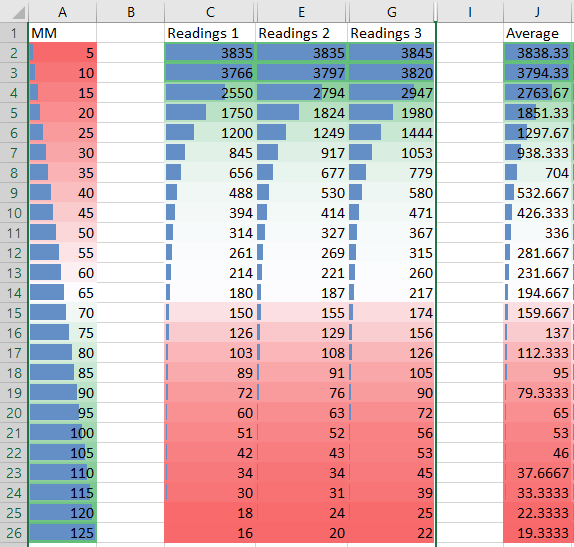
\includegraphics[width=\textwidth,height=\textheight,keepaspectratio]{irRange}
	\subsubsection{Repeatability \& Reliability}
	\subsubsection{Similarity}
\subsection{Data Visualised}
	\subsubsection{range of distances}
	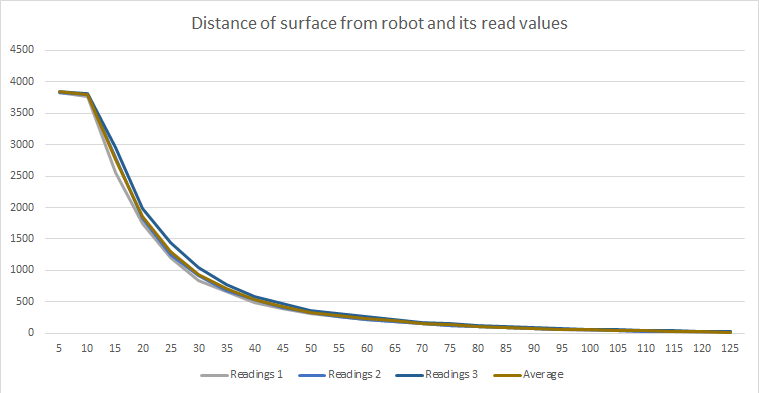
\includegraphics[width=\textwidth,height=\textheight,keepaspectratio]{irRangeLineGraph}
	\subsubsection{Repeatability \& Reliability}
	\subsubsection{Similarity}
\subsection{Discussion}
	\subsubsection{range of distances}
		From the data we can determine the range of useful distances are from 10mm to around 120mm where the difference between the sensor values for different distances is not significant.
		
		We can also determine a function for the relationship between the sensor reading and actual distance in mm. By logging the sensor reading we end up with a reasonably straight line to fit the y = mx + c model which allows us to calculate a gradient and a y intercept.
		
		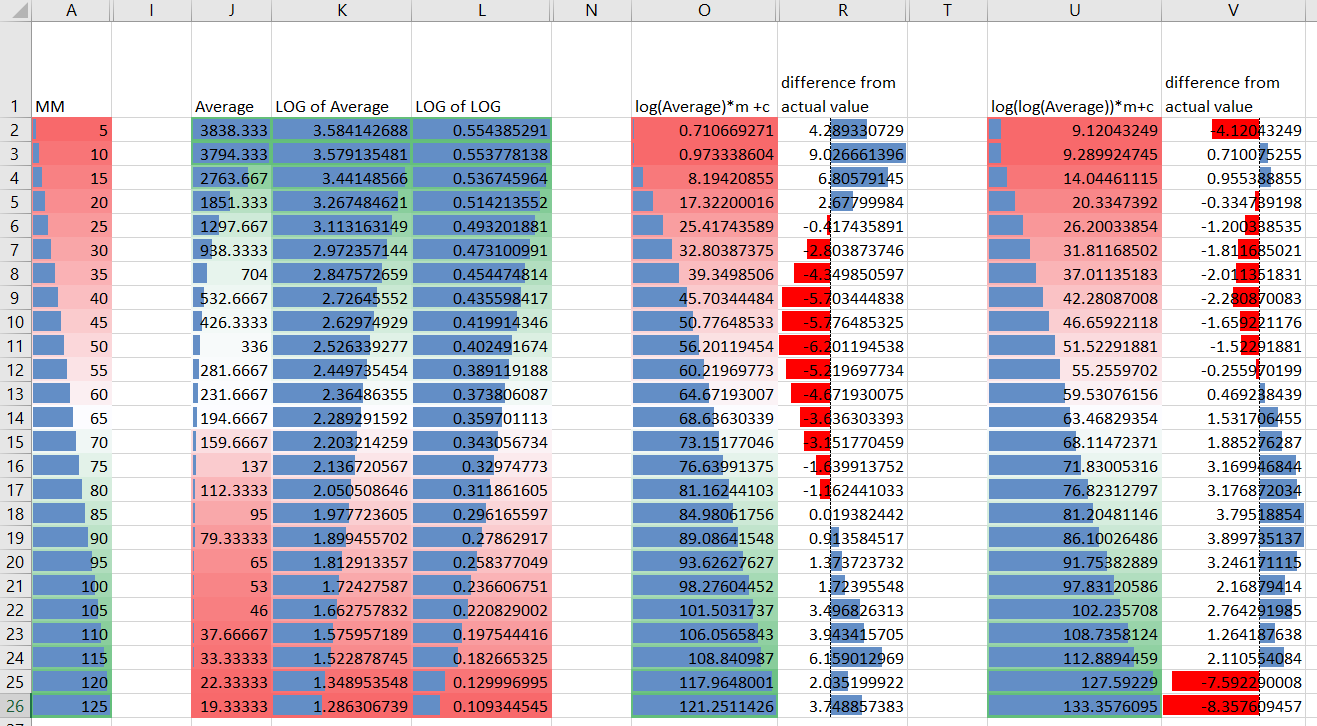
\includegraphics[width=\textwidth,height=\textheight,keepaspectratio]{irRangeLineData}
		
		From the data we can see that the distance from the actual value is less for the log of log and from this we can determine that the relationship.
		\begin{quotation}
			Obstacle distance in mm = log(log(sensor value))*-M+C
		\end{quotation}
		For this set of data the gradient is -279 and the intercept is 163 which used a white obstacle. The experiment was re done with a black obstacle and gradient came out at -198 and intercept at 110. As these are both the extreme cases of objects reflection and light absorption, an average was take to determine the distance more reliably at a gradient of -238 and intercept of 136.
	\subsubsection{Repeatability \& Reliability}
	\subsubsection{Similarity}

\section{Encoders}
\subsection{Programming}
\begin{lstlisting}[language=C,frame=single]
void encodersDataGathering(int power){
 FA_SetMotors(power,power);
 FA_DelayMillis(500 + power*10);
 int i;
 for(i = 0;i<5;i++){
  FA_ResetEncoders();
  FA_DelayMillis(1000);
  FA_LCDNumber(FA_ReadEncoder(1), 25*i, 
    1, FONT_NORMAL, LCD_OPAQUE);
  FA_LCDNumber(FA_ReadEncoder(0), 25*i, 
    12, FONT_NORMAL, LCD_OPAQUE);
 }
 FA_SetMotors(0,0);
}

int main(){
 FA_RobotInit();
 FA_LCDBacklight(50);
 int power = 0;

 while(1){  
  if(FA_ReadSwitch(0)){
   FA_LCDClear();
   encodersDataGathering(power);
  }
  if(FA_ReadSwitch(1)){
   FA_LCDNumber(power, 0, 
    24, FONT_NORMAL, LCD_OPAQUE);
   power = power + 10;
   FA_DelayMillis(200);
  }
 }
}

\end{lstlisting}
\subsection{Data Acquistion}
	\subsubsection{Range of power}
	\subsubsection{Repeatability}
	\subsubsection{Similarity}
\subsection{Data Captured}
	\subsubsection{Range of power}
	\subsubsection{Repeatability}
	\subsubsection{Similarity}
\subsection{Data Visualised}
	\subsubsection{Range of power}
	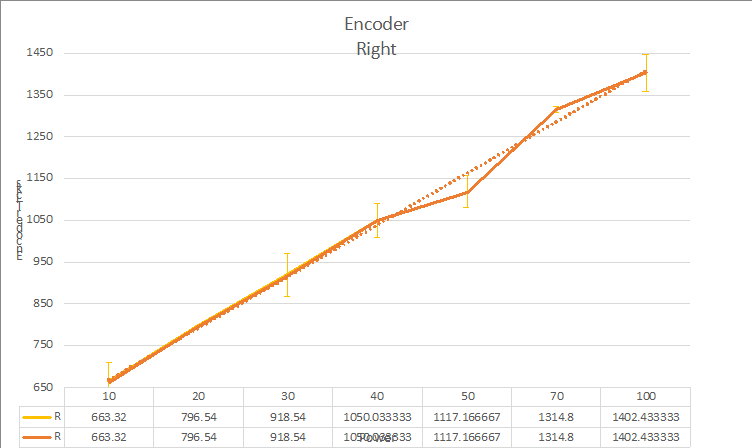
\includegraphics[width=\textwidth,height=\textheight,keepaspectratio]{EncodersRight}
	
	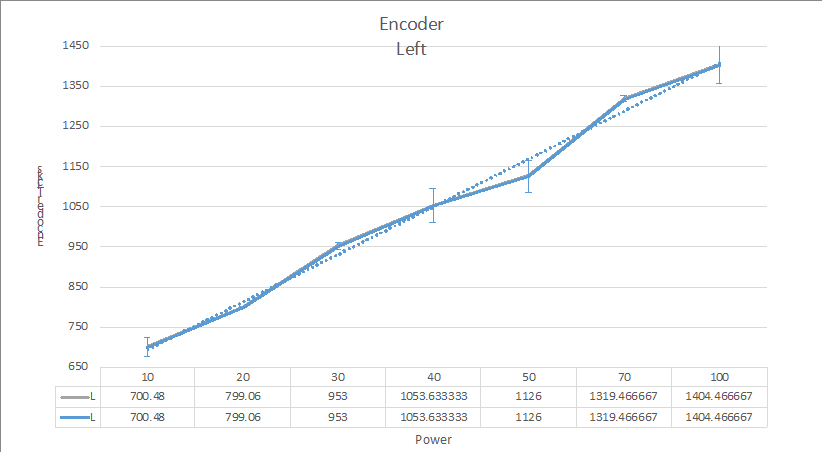
\includegraphics[width=\textwidth,height=\textheight,keepaspectratio]{EncodersLeft}
	\subsubsection{Repeatability}
	\subsubsection{Similarity}

\subsection{Discussion}
	\subsubsection{Range of power}
	\subsubsection{Repeatability}
	\subsubsection{Similarity}

\clearpage
\addcontentsline{toc}{section}{REFERENCES}
\begin{thebibliography}{5}
\bibitem{Formula all-code} \emph{Formula AllCode Robot}
\url{https://www.matrixtsl.com/allcode/formula/}
\bibitem{in-robot api} \emph{in-robot API}
allcode\_api.h \& allcode\_api.o
Pete Todd \& Laurence Tyler 1.1
\end{thebibliography}
\clearpage

\label{thelastpage}
\end{document}